\documentclass{article}
\title{
    \LARGE Pineapple Planner\\[0.2em]
    \Large Agile Development Project Report
}
\author{Max Sellick, Varvara Aladyina, Deinoras Krasauskas,\\ Azhaf Kahn, Simon Ostini}
\date{March 2025}

\usepackage{graphicx}
\graphicspath{{images/}}

\usepackage{booktabs}
\usepackage{ulem}
\usepackage{float}
\usepackage[utf8]{inputenc}
\usepackage[english]{babel}
\usepackage[style=ieee]{biblatex}
\addbibresource{references/references.bib}
\usepackage{csquotes}
\usepackage[utf8]{inputenc}
\usepackage{hyperref}
\hypersetup{
    colorlinks=true,
    linkcolor=black,
    filecolor=magenta,
    urlcolor=blue,
}
\usepackage{listings}

\lstset{
    language=[Sharp]C,
    breakatwhitespace=false,         
    breaklines=true,                 
    captionpos=b,                    
    keepspaces=true,                 
    numbers=left,                    
    numbersep=5pt,                  
    showspaces=false,                
    showstringspaces=false,
    showtabs=false,                  
    tabsize=4
}

\usepackage{multirow, makecell}
\usepackage{pgfplots}
\pgfplotsset{compat=1.18}
\usepackage{caption}
\usepackage{calculator}
\usepackage{calculus}
\usepackage{geometry}
\geometry{
    a4paper,
    left=30mm,
    right=30mm,
    top=25mm,
    bottom=30mm,
    headheight={90pt},
}
\usepackage[shortlabels]{enumitem}

\usepackage{enumitem}
\usepackage{tabularx}
\usepackage{booktabs}

\addto\captionsenglish{\renewcommand{\listfigurename}{Plots}}
\addto\captionsenglish{\renewcommand{\listtablename}{Tables}}

\begin{document}
\begin{figure}[ht!]
  \minipage{0.76\textwidth}
  
\includegraphics[width=7cm]{images/hkr.png}
  \label{title}
  \endminipage
  \minipage{0.32\textwidth}
  \endminipage
\end{figure}

\vspace{0.8cm}
\large

\textbf{{\let\newpage\relax\maketitle}}

\begin{center}
  \vfill
  \small{Kristianstad University | SE-291 88 Kristianstad | +46 44 250 30 00 | www.hkr.se}
\end{center}

\thispagestyle{empty}

\newpage

\makeatletter
\renewcommand{\abstractname}{\vspace{-\baselineskip}}
\begin{abstract}
  \large
  \noindent\textbf{Title}\\
  Pineapple Planner\\[1em]
  \noindent\textbf{Subtitle}\\
  Agile Development Project Report\\[1em]
  \textbf{Programme}\\
  Software Development\\[1em]
  \textbf{Authors}\\
  Max Sellick, Varvara Aladyina, Deinoras Krasauskas, Azhaf Khan, Simon Ostini\\[1em]
  % Abstract\\[1em]
  \textbf{Keywords}\\
  Agile, Scrum, Project idea\\[1em]
\end{abstract}
\makeatother

\newpage

\tableofcontents
\thispagestyle{empty}

\newpage
\listoffigures
\lstlistoflistings
\listoftables

\newpage

\section{Introduction}
%✅<Instructions: Write an introduction to your application and its purpose. Also include screenshot>
Time management is a challenge for individuals that have multiple responsibilities across work, studies, and personal life, what leads to increased stress and decreased productivity.
Study-related stress and disruption of mental health may take origins from procrastination which is quite common among individuals with poor time management skills \cite{ nayak2019impact}.
Traditional calendars and to-do lists, while useful, may not provide the comprehensive support needed to manage these demands effectively \cite{bek2014study}.\\
PineapplePlanner is a Windows application designed to serve as an intuitive to-do list integrated within a calendar which aims to minimize stress to help completing daily tasks and refines personal productivity. The application is focused on improving mental health stability with focus on SDG 4.3.2 \cite{worldhealthorganisation_2024_sdg}.
PineapplePlanner enables users to create and manage tasks efficiently by specifying a start and finish date, selecting a priority level (high, medium, low, or no priority), and providing a descriptive task name before submitting it to the calendar.
With a user-friendly interface, multiple language translation, and AI-powered assistance, PineapplePlanner simplifies task creation by allowing users to generate tasks through natural language input—simply describing what they need to do, and the AI will automatically create and categorize the task for them.
For those who prefer a more hands-on approach, PineapplePlanner also allows users to manually input their tasks, giving them full control over their scheduling.
This makes the process even more seamless for individuals who feel overwhelmed by a heavy workload or numerous responsibilities, offering a structured and organized approach to task management.
By visually mapping out tasks within a calendar, users can prioritize effectively, track deadlines, and stay on top of their commitments with greater ease and clarity.
Whether users need to focus on urgent tasks or simply keep track of general activities, PineapplePlanner provides the flexibility to accommodate different levels of importance.

\begin{figure}[H]
  \centering
  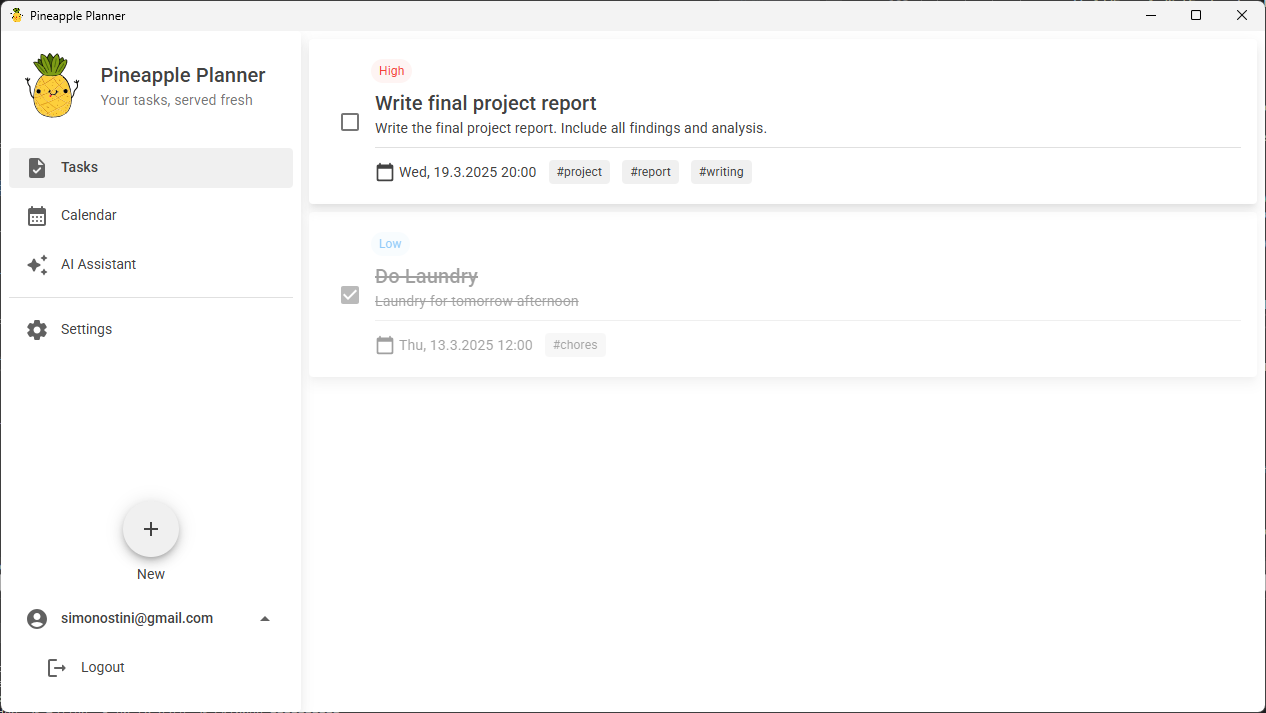
\includegraphics[width=1\textwidth]{images/pineapple_planner_screenshot_home.png}
  \label{Infrastructure proposal}
  \caption{Pineapple Planner home page screenshot}
\end{figure}

\subsection{Source code}
The entire project source code is open source in a public Github repository \href{http://www.github.com/b3h3m0th/pineapple-planner}{here (github.com/b3h3m0th/pineapple-planner)}.

\subsection{Restrictions}
%< ✅Instructions: List any restrictions that you think is worth mentioning.>
The only restriction PineapplePlanner has is that users must have a Google account to sign up or sign in. However, since most people already have one, this is hardly an issue.
\subsection{Enhancements}
%< Instructions: Explain possible extra features that you plan to implement into your application. If you have no extra features, you can remove this 1.2 section.>

%The possible extra features we planned to implement or that has been implemented was custom usernames for users which was already implemented, dark-mode option in settings which transforms the application to dark-mode for users who would prefer to have it that way. AI was another feature that got implemented to help users create tasks faster. Not yet implemented features were Notification features in settings that would allow users to enable/disable notifications, Language option in settings for users whom do not understand english or would rather prefer have it in another language.

Throughout the four sprints, we thought about several possible features that could be done. However, due to time constraints, we were unable to implement them. Some of these planned features are:

\begin{enumerate}
  \item Notification Settings: Users can enable or disable notifications based on their preferences;
  \item Burnout reminder:  If a user schedules too many deadlines in a single day, PineapplePlanner will suggest redistributing tasks to prevent overwhelming workloads;
  \item Gamification: Users can assign points to tasks and earn rewards upon completion, creating a more engaging task management experience;
  \item Day Streaks: To motivate user to use PineapplePlanner, a streak system would encourage user to complete tasks daily.
  \item Recurring Tasks: A feature that allows users to set tasks to repeat at specified intervals;
  \item Family groups: Users can create shared groups to manage tasks and events collaboratively with family members or friends.
\end{enumerate}


\section{Requirements}

%<Instructions: In the table below, add a list of all requirements for your application. They shall be numbered from 1..N. Each requirement has a short name and a longer description. Estimate how many hours it will take to complete the task for 1 person working with the task (man hours). At the start of a new iteration, you shall fill in estimated man hours to complete a task (EMH). This is your initial estimate – do NOT change it later. At the end of a weekly iteration, you shall fill in the actual man hours spent (AMH). In this way, you will establish a record that shows how good you are at estimating tasks, and you will hopefully learn from it and become better at next week’s estimate. Then prioritize the feature: How important is it? 1 for most important. 10 for least important. >
%Table 1 below lists all the requirements for this project. The time estimated (EMH) and time spent on a task (AMH) is measured in man hours. The prio column lists feature priorities where Prio 1 is highest priority and Prio 10 is lowest priority

\begin{table}[H]
  \centering
  \begin{tabularx}{\textwidth}{|c|c|X|c|c|c|}
    \toprule
    \textbf{Nr} & \textbf{Req. Name}         & \textbf{Req. Description}                                                    & \textbf{EMH} & \textbf{AMH} & \textbf{Prio} \\
    \hline
    1           & Log in                     & Allows users to log in to see their personal tasks.                          & 10           & 30           & 10            \\    \hline
    2           & Log out                    & Allows users to log out to secure their information                          & 1            & 5            & 10            \\    \hline
    3           & Task creation              & Allows users to create a task with a name, description and a deadline        & 7            & 30           & 10            \\    \hline
    4           & Edit task                  & The tasks can be edited and marked as completed.                             & 15           & 30           & 8             \\    \hline
    5           & Task prioritization        & Tasks have priorities: low, medium and high.                                 & 5            & 30           & 6             \\    \hline
    6           & View tasks in the calendar & Tasks(events) are displayed in calendar view.                                & 10           & 50           & 10            \\    \hline
    7           & Add tasks in the calendar  & Integrates task creation directly into the calendar view                     & 5            & 20           & 6             \\    \hline
    8           & Tags                       & Provides tagging functionality for easier management.                        & 7            & 15           & 5             \\    \hline
    9           & Dark theme                 & Offers a dark theme option in the settings                                   & 5            & 20           & 3             \\    \hline
    10          & AI                         & Integrates AI (Gemini) to assist users in generating tasks and events        & 20           & 30           & 3             \\\hline
    11          & Languages                  & Allows users to switch languages to use the app in their preferred languages & 15           & 20           & 3             \\
    \bottomrule
  \end{tabularx}
  \caption{Requirements}
  \label{Requirements with EMH, AMH, and priority}
\end{table}

\section{Design and Implementation}
%< Instructions: Describe your design in this chapter.
%List one class per sub chapter and add some simple class diagrams to illustrate relations (inheritance and/or associations) between the main classes.>

The application implementation is far to large to list and explain every single class.
As the application is built with the object oriented language C\verb|#| almost everything is a class.
Thus, an explanation class-per-class does not really add any value.
Some crucial classes with different use cases are explained in the following sections.
\\
The entire project is contained in one .NET solution.
This solution is divided into different projects for organization purposes.
For instance, we have a class library project for all user interface related code, a class library for communication with the database and a class library for all entity classes and enums.

\subsection{PineapplePlanner.Domain.Entities.Entry}

The \verb|Entry| class is our base entity class for user entries.
There are two child classes \verb|Task| and \verb|Event| that are derived from \verb|Entry|.

The class itself has a \verb|[FirestoreData]| attribute which enables instances to be stored in the Firebase Firestore database.
All properties with a \verb|[FirestoreProperty]| are marked to be stored in the Firestore.

\lstinputlisting[label=PineapplePlanner.Domain.Entities.Entry, caption=PineapplePlanner.Domain.Entities.Entry]{snippets/Entry.cs}
\bigbreak

\subsection{PineapplePlanner.Application.Repositories.BaseRepository}

\verb|BaseRepository| is a generic class that implements the \verb|IBaseRepositor| according to the common Repository pattern.
All other Repository are derived from the \verb|BaseRepository| which has shared CRUD implementations.
The \verb|BaseRepository| accepts a generic argument which decides what Firestore collection should taken into account.

\lstinputlisting[label=PineapplePlanner.Application.Repositories.BaseRepository, caption=PineapplePlanner.Application.Repositories.BaseRepository]{snippets/BaseRepository.cs}
\bigbreak

\subsection{PineapplePlanner.Domain.UnitTests.Shared.ResultBaseTests}

The \verb|ResultBaseTests| class contains unit tests for our custom \verb|ResultBase| class that is used for error handling throughout the entire project.
The unit tests are implemented using the .NET testing library XUnit.
Each unit test is declared with a \verb|Fact| attribute.

\lstinputlisting[label=PineapplePlanner.Domain.UnitTests.Shared.ResultBaseTests, caption=PineapplePlanner.Domain.UnitTests.Shared.ResultBaseTests]{snippets/ResultBaseTests.cs}
\bigbreak

\subsection{UML diagram of partial PineapplePlanner.Domain namespace}

\begin{figure}[H]
  \centering
  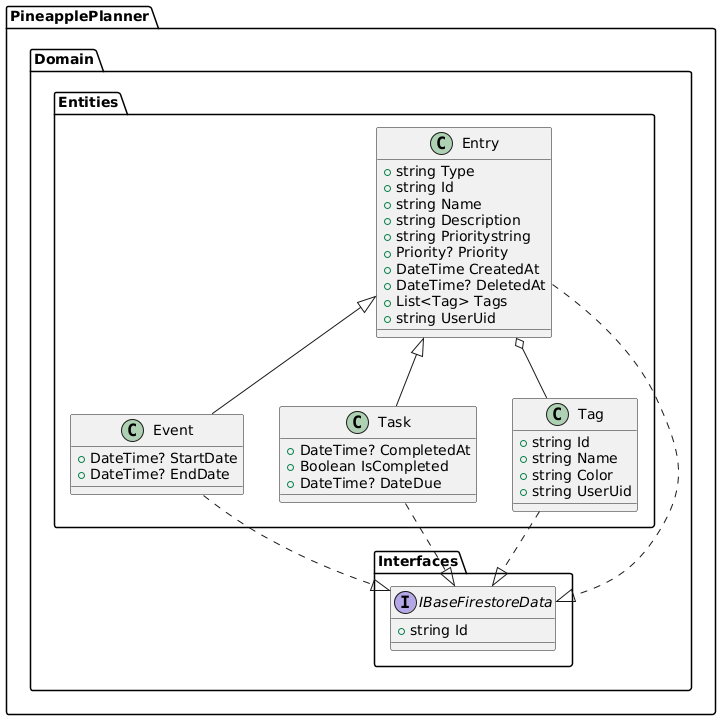
\includegraphics[width=1\textwidth]{images/domain_uml_diagram.png}
  \label{Partial PineapplePlanner.Domain UML diagram}
  \caption{Partial PineapplePlanner.Domain UML diagram}
\end{figure}

\clearpage
\section{Test Results}
Table 2 below contains the current status of implemented and tested requirements.
%<Instructions: This table shall map 1-1 to the table in Chapter 2. The test result for each requirement shall be one of the following: NOT IMPLEMENTED, PASSED or FAILED.>

\begin{table}[H]
  \centering
  \begin{tabularx}{\textwidth}{|c|X|c|}
    \toprule
    \textbf{Nr} & \textbf{Req. Name}         & \textbf{Test result} \\
    \hline
    1           & Log in                     & Not Implemented      \\    \hline
    2           & Log out                    & Not Implemented      \\    \hline
    3           & Task creation              & Not Implemented      \\ \hline
    4           & Edit task                  & Not Implemented      \\    \hline
    5           & Task prioritization        & Not Implemented      \\    \hline
    6           & View tasks in the calendar & Not Implemented      \\    \hline
    7           & Add tasks in the calendar  & Not Implemented      \\    \hline
    8           & Tags                       & Not Implemented      \\ \hline
    9           & Dark theme                 & Not Implemented      \\    \hline
    10          & Tags                       & Not Implemented      \\\hline
    11          & AI                         & Not Implemented      \\\hline
    12          & Languages                  & Not Implemented      \\\hline
    13          & Domain entities            & Implemented          \\\hline
    14          & Error handling             & Implemented          \\
    \bottomrule
  \end{tabularx}
  \caption{Test results}
  \label{results}
\end{table}

\section{Summary and Conclusion}
This chapter contains a summary and conclusion of the work that was carried out in this project as well as reflections and thoughts about working methods and challenges.

\subsection{Weekly Progress}
Below is a short summary of what was done each week.

\subsubsection{Week 1}
In week 1, we made significant strides in setting up the foundation for our project.
We established the GitHub repository, integrated Jira for streamlined project management, and configured Firebase for backend support.
Additionally, we implemented user authentication and conducted a thorough code refactor to enhance efficiency and maintainability

\subsubsection{Week 2}
In Week 2, we focused on refining the user experience and adding key features.
The UI was designed and implemented, email verification was integrated for secure access, and a custom logo was created and applied.
Furthermore, essential features such as the calendar, settings panel, and to-do list were developed and implemented to enhance functionality and usability.

\subsubsection{Week 3}
In Week 3, we focused on improving functionality and stability.
Unit tests were added to ensure reliability, minor issues were fixed for a smoother experience, and dark mode was implemented to enhance usability.
We also introduced a tagging system for better organization and navigation.

\subsubsection{Week 4}
In Week 4, we made improvements to both functionality and project organization.
The AI assistant was enhanced, and Git branch protection was set up to maintain code integrity.
Additional settings features were implemented, localization was introduced, and various codebase warnings were cleaned up.
Finally, we started working on the final report.

\subsection{Difficulties and challenges}
Below is a list of notable challenges that came up during this project and that took a long time to solve.

\subsubsection{Blazor WPF wrapper}
One significant challenge we faced several times was the fact that we decided to implement our Blazor SSR web application within a WPF wrapper to be ran as a desktop application.
Having a web based application is very comfortable for development, especially when it comes to building user interfaces. Also you can always fallback to use JavaScript as the app runs in the browser.
On the other hand, having a WPF wrapper limited us when implementing certain features.\\
For instance, redirects that were necessary for the authentication with Firebase turned out to be rather difficult.

\subsubsection{Dependency Injection issues}
Blazor and WPF both have their own dependency injection frameworks and ensuring proper integration between the two required some trial and error.
Some services that worked seamlessly within Blazor did not behave as expected when instantiated inside the WPF wrapper.
For example, singleton services shared between Blazor and WPF sometimes led to unintended issues.
The whole services setup took quite some time.

\subsubsection{Lack of console outputs for debugging}
Another major difficulty we encountered was the lack of direct console output when running the Blazor application within the WPF wrapper.
Usually, web applications benefit from browser developer tools, in particular the console outputs.
However, within the WPF environment, there was neither a .NET console nor a browser console available making debugging significantly harder.
We often ended up rendering output to the user interface for testing.

\subsubsection{Firebase API Quota Exceeded}
During development and testing, we occasionally exceeded Firebase's API quota.
This typically happened when we testing extensively in a short period or when our application accidentally fell into an endless request loop.
We had to be extremely careful not to get stuck in infinite render loops.
Otherwise we had to wait one day for the firebase cooldown to continue development.

\subsection{Correctness of time estimates}
%<Instructions: Look back on your time estimates and discuss your results. How accurate were they? What have you learned about time estimates and how can you get better in next project?>

When estimating the time required for each task, we aimed to provide realistic approximations based on complexity and priority. After reviewing our actual development process, we found that most predictions were not that accurate and we spent nearly twice as much time as initially estimated. However, the additional time was spent mostly for refining features, improving functionalities and smoothing out the code.\\
Time estimates are helpful in developing, since it's crucial to have approximate measurement of time that tasks will take. However, the less defined the task is, the less precise predictions are made. For future projects, we plan to track time more precisely by tracking AMH and breaking down complex tasks into smaller, more manageable subtasks. Also, Jira might help to improve timetracking better by grouping related tasks into Epics. This approach will help improve the accuracy of our time predictions and optimize workflow efficiency.

\subsection{Priority decisions}
%<Instructions: Look back on your feature priority settings. Did you prioritize the right features? Did you succeed to deliver the highest prioritized features? Did you disagree with the examiner on some features? Have you learned anything about setting priorities?>

Looking back at the feature priorities we set a month ago for our first 6 requirements, we can see that we successfully delivered 4 out of 6. However, we did not complete the last two requirements, which were ranked as medium and low priority. Instead, we've created other features such as AI, tags, languages, dark theme, change of the username, etc. during 2 sprints that we had.\\
At the first PM, the examiner recommended starting with the 3rd requirement (log in/out user), and we followed that advice. As a result, the remaining features were easier to implement.\\
We learned that setting priorities at the start of the project is important for a quick start in agile development. While focusing on high-priority features, it's also important to keep in mind that lower-priority features may change significantly during subsequent sprints.\\

\begin{table}[H]
  \centering
  \begin{tabularx}{\textwidth}{|l|X|l|}
    \toprule
    \textbf{Nr} & \textbf{Requirement item}                                 & \textbf{Priority (High/Medium/Low)} \\
    \hline
    R1          & The user shall be able to inspect their tasks.            & High                                \\
    \hline
    R2          & The user shall be able to manage their tasks.             & High                                \\
    \hline
    R3          & The user shall link their task data to their account.     & High                                \\
    \hline
    R4          & The user shall be able to prioritize tasks.               & Medium                              \\
    \hline
    R5          & \sout{The user shall be able to set recurring tasks.}     & Medium                              \\
    \hline
    R6          & \sout{The user shall be able to set reminders for tasks.} & Low                                 \\
    \bottomrule
  \end{tabularx}
  \caption{Requirement items from previous report}
  \label{Requirement items from previous report}
\end{table}

\subsection{Conclusion}
%<Instructions: Look back on the whole project. Here you can write a bit more freely about your thoughts on this project. What was your overall experience? How was the teamwork? What did you learn? Can you list some points that you will do better in next project? Other thoughts. >
Overall, it was a rewarding experience to do this project, PineapplePlanner, with the team. Working with experienced programmers and relatively new ones was slightly challenging because of the gap in knowledge. It was hard to keep up for some team members, but at the same time it also provided a valuable experience to work with completely new frameworks, new programming language, and new development environment. \\
Despite the challenges, the diversity of skills in the team had its advantages. The experienced programmers offered guidance, motivation, and feedback, and other team members worked in comfortable workspace, refactoring and suggesting improvements for PineapplePlanner. This helped create a collaborative environment where we could learn from each other.\\
For the next project it would be nice to have more frequent discussions in the team, because the more we talk, the fewer misunderstandings and conflicts we’ll have regarding the work. Clearer objectives would be created and members wouldn't be awkward to asking for help in the case of problems. We would also focus on better time management and setting realistic expectations for task completion. This could help streamline the process and ensure that we make steady progress without rushing. Overall, this project was a great learning experience, and I’m looking forward to applying the lessons learned to future teamwork.
\clearpage

\section{References}
\nocite{*}
\printbibliography[heading=none]

\end{document}
